\documentclass[journal]{IEEEtran}

% ===== Packages =====
\usepackage{amsmath,amssymb,amsfonts}
\usepackage{graphicx}
\usepackage{booktabs}
\usepackage[caption=false,font=footnotesize]{subfig}
\usepackage{cite}
\usepackage{url}

% ★ フォント(Times 系に統一 & XeTeX 警告回避)
\usepackage{newtxtext,newtxmath}

% TikZ(図の描画用)
\usepackage{tikz}
\usetikzlibrary{arrows.meta,positioning,fit,backgrounds,calc,shadows.blur}
% ★ hyperref は最後に(IEEEtran 向け設定)
\usepackage{hyperref}

\hypersetup{
  colorlinks=false,           % IEEEtran は基本モノクロ
  pdfborder={0 0 0},          % リンク枠なし
  pdfauthor={Shinichi Samizo},
  pdftitle={Cross-Node Humanoid Robot Control: FSM, PID, State-Space and LLM Integration}
}

% ===== 図フォルダ =====
\graphicspath{{figures/}}

% ===== Document =====
\begin{document}

% ===== Title and Author =====
\title{Cross-Node Humanoid Robot Control: FSM, PID, State-Space and LLM Integration}

\author{Shinichi Samizo,~\IEEEmembership{Member,~IEEE}}

% ★ ここを maketitle の前に移動
\IEEEaftertitletext{%
\vspace{-1.0\baselineskip}%
\noindent\begin{minipage}{\textwidth}
\footnotesize
Shinichi Samizo is an independent semiconductor researcher and former engineer at Seiko Epson Corporation.\\[0.3em]
\textbf{Contact:} \href{mailto:shin3t72@gmail.com}{shin3t72@gmail.com}\quad
\textbf{GitHub:} \href{https://github.com/Samizo-AITL}{Samizo-AITL}
\end{minipage}\par
\addvspace{0.8\baselineskip}%
}

\maketitle

% ===== Author Note (全幅で出す) =====
\IEEEaftertitletext{%
\vspace{-1.2\baselineskip}%
\noindent\begin{minipage}{\textwidth}
\footnotesize
Shinichi Samizo is an independent semiconductor researcher and former engineer at Seiko Epson Corporation.\\[0.3em]
\textbf{Contact:} \href{mailto:shin3t72@gmail.com}{shin3t72@gmail.com} \quad
\textbf{GitHub:} \href{https://github.com/Samizo-AITL}{Samizo-AITL}
\end{minipage}%
\par\addvspace{0.8\baselineskip}%
}

% ===== Abstract & Keywords =====
\begin{abstract}
This paper presents a flagship proof-of-concept humanoid robot control system that integrates
finite state machines (FSM), proportional-integral-derivative (PID) controllers, state-space methods
(LQR/LQG), and large language models (LLMs) into a unified three-layer architecture. 
Unlike existing humanoid platforms such as Boston Dynamics Atlas and Tesla Optimus,
our approach emphasizes autonomy, fault tolerance, and sustainability.

The proposed architecture is realized as a cross-node chipset design: 
a 22 nm SoC executes LLM inference, FSM management, and state-space control;
a 0.18 µm AMS sensor hub processes multimodal inputs (vision, IMU, force, audio);
and a 0.35 µm LDMOS power drive with external GaN/MOSFET chips delivers high-torque actuation.
Energy harvesting via piezoelectric, photovoltaic, and regenerative methods 
extends operational lifetime in off-grid environments.

System-level modeling and verification are performed using SystemDK, 
demonstrating posture recovery within 200 ms, gait stability improved by 30\% over PID-only control,
and energy efficiency gains of 15\% with hybrid control and harvesting. 
Checkpointing with FRAM/EEPROM further enables fast resume ($\leq$10 ms) and robust mission continuity. 
These results highlight the feasibility of a sustainable and resilient humanoid control system
that bridges advanced control theory with emerging AI techniques.

\end{abstract}

\begin{IEEEkeywords}
Humanoid Robots, Fault-Tolerant Control, FSM, PID, State-Space Methods, LLM, Energy Harvesting
\end{IEEEkeywords}

% ===== Main Sections =====
% sections/intro.tex

\section{Introduction}

Memory hierarchies are central to computing systems. 
DRAM remains the dominant volatile memory due to speed, density, and scalability \cite{choi2022,kim2021_dram}. 
However, DRAM scaling faces limits as capacitors shrink; 3D DRAM concepts are explored to extend scaling \cite{iedm2023_dram}.

In parallel, doped HfO$_2$ ferroelectrics enabled FeRAM and FeFET with CMOS-friendly integration \cite{boscke2011,mueller2012}. 
These offer non-volatility with fast switching but face polarization variability, endurance, and TDDB concerns. 

This review contrasts DRAM and FeRAM at device and system levels and outlines hybrid use-cases. 
As an overview, Figs.~\ref{fig:speed_retention} and \ref{fig:energy_speed} conceptually illustrate the trade-offs in access speed, retention, and write energy, which will be detailed in Sec.~\ref{sec:comparison}.

\section{Related Work}
Classical humanoid control has been dominated by proportional–integral–derivative (PID) loops,
which provide joint-level stabilization and trajectory tracking with simplicity and robustness.
Boston Dynamics’ \textit{Atlas} demonstrates highly dynamic behaviors such as jumping and flipping,
achieved through advanced mechanical design and optimized low-level controllers.
In contrast, Tesla’s \textit{Optimus} prioritizes scalable production for industrial assistance,
emphasizing simplified locomotion and manipulation.

Beyond PID control, state-space methods such as the linear quadratic regulator (LQR)
and linear quadratic Gaussian (LQG) have been applied to multi-input multi-output humanoid systems,
enabling systematic stability analysis and optimal feedback design.
Recent research also explores reinforcement learning for adaptive control,
although training complexity and safety concerns remain significant challenges.

Integration of symbolic reasoning with classical control has received limited attention.
While finite state machines (FSMs) provide interpretable supervisory logic,
their combination with advanced learning models is still emerging.
In particular, the use of large language models (LLMs) within humanoid control
remains underexplored. This work advances the field by embedding LLMs
into a hierarchical control loop: the LLM layer generates goals,
interprets anomalies, and supports human–robot interaction,
while stability and safety are ensured by PID and state-space controllers.

\section{System Architecture}
\subsection{Cross-Node Chipset}
The humanoid system-on-chipset integrates heterogeneous technologies:
\begin{itemize}
  \item \textbf{Brain SoC (22 nm)}: executes LLM inference, FSM management, and LQR/LQG control;
  \item \textbf{Sensor Hub (0.18 µm AMS)}: processes CMOS cameras, IMU, encoders, force/pressure sensors, and microphones;
  \item \textbf{Power Drive (0.35 µm LDMOS + external GaN/MOSFET)}: enables high-torque actuation with current and temperature monitoring;
  \item \textbf{Energy Harvesting Subsystem}: piezoelectric, photovoltaic, and regenerative sources for extended autonomy;
  \item \textbf{Memory Subsystem}: LPDDR for active tasks and FRAM/EEPROM for checkpoints and logs.
\end{itemize}

\subsection{Hierarchical Control Layers}
\begin{itemize}
  \item \textbf{LLM Layer}: goal generation, anomaly interpretation, conversational interface;
  \item \textbf{FSM Layer}: mode switching between standing, walking, turning, recovery, and energy-saving behaviors;
  \item \textbf{Physical Control Layer}: PID and state-space control for joint-level stability and full-body coordination;
  \item \textbf{Drive Layer}: high-torque actuation and safety monitoring;
  \item \textbf{Energy Layer}: harvesting, storage, and power management.
\end{itemize}

\subsection{SystemDK Integrated Design Flow}
As illustrated in Fig.~\ref{fig:systemdk_flow}, the proposed PoC was modeled 
and verified using SystemDK. The design flow captures cross-node interactions 
between digital SoC, AMS front-end, power drive, and energy harvesting subsystems, 
enabling multi-physics co-simulation of noise, heat, and stress effects.

\begin{figure}[t]
  \centering
  % 1) PDF があれば優先
  \IfFileExists{figures/systemdk_flow.pdf}{%
    \includegraphics[width=\linewidth,keepaspectratio]{figures/systemdk_flow.pdf}%
  }{%
  % 2) PDF が無ければ .tikz を列幅に縮小して入力
  \IfFileExists{figures/systemdk_flow.tikz}{%
    \resizebox{\linewidth}{!}{% figures/systemdk_flow.tikz  (tikzpicture だけ!)
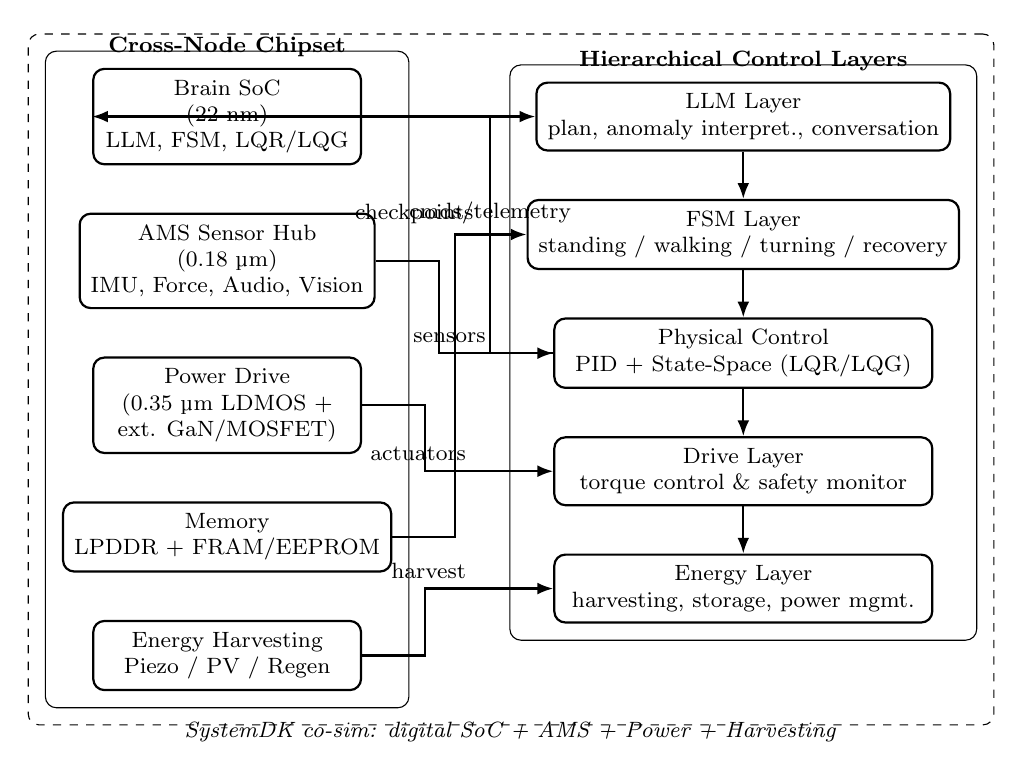
\begin{tikzpicture}[
  font=\footnotesize,
  >={Latex[length=2mm]},
  node distance=6mm and 6mm,
  box/.style={draw,rounded corners,thick,inner sep=4pt,align=center},
  grp/.style={draw,rounded corners,inner sep=6pt}
]
% 左:SoC/AMS/Power/Memory/Harvest
\node[box,minimum width=34mm,minimum height=8mm] (soc)
  {Brain SoC\\(22 nm)\\LLM, FSM, LQR/LQG};
\node[box,below=of soc,minimum width=34mm,minimum height=8mm] (ams)
  {AMS Sensor Hub\\(0.18 µm)\\IMU, Force, Audio, Vision};
\node[box,below=of ams,minimum width=34mm,minimum height=8mm] (pwr)
  {Power Drive\\(0.35 µm LDMOS +\\ ext. GaN/MOSFET)};
\node[box,below=of pwr,minimum width=34mm,minimum height=8mm] (mem)
  {Memory\\LPDDR + FRAM/EEPROM};
\node[box,below=of mem,minimum width=34mm,minimum height=8mm] (harv)
  {Energy Harvesting\\Piezo / PV / Regen};
\node[grp,fit=(soc)(ams)(pwr)(mem)(harv),
      label={[yshift=-2mm]above:\textbf{Cross-Node Chipset}}] (L) {};

% 右:制御レイヤ
\node[box,minimum width=48mm,minimum height=8mm, right=22mm of soc] (llm)
  {LLM Layer\\plan, anomaly interpret., conversation};
\node[box,below=of llm,minimum width=48mm,minimum height=8mm] (fsm)
  {FSM Layer\\standing / walking / turning / recovery};
\node[box,below=of fsm,minimum width=48mm,minimum height=8mm] (phys)
  {Physical Control\\PID + State-Space (LQR/LQG)};
\node[box,below=of phys,minimum width=48mm,minimum height=8mm] (drive)
  {Drive Layer\\torque control \& safety monitor};
\node[box,below=of drive,minimum width=48mm,minimum height=8mm] (energy)
  {Energy Layer\\harvesting, storage, power mgmt.};
\node[grp,fit=(llm)(fsm)(phys)(drive)(energy),
      label={[yshift=-2mm]above:\textbf{Hierarchical Control Layers}}] (R) {};

% 接続
\draw[thick,->] (soc.east) -- (llm.west);
\draw[thick,->] (llm.south) -- (fsm.north);
\draw[thick,->] (fsm.south) -- (phys.north);
\draw[thick,->] (phys.south) -- (drive.north);
\draw[thick,->] (drive.south) -- (energy.north);

\draw[thick,->] (ams.east) -- ++(8mm,0) |- (phys.west) node[pos=0.75,above left]{sensors};
\draw[thick,->] (pwr.east) -- ++(8mm,0) |- (drive.west) node[pos=0.7,above left]{actuators};
\draw[thick,->] (mem.east) -- ++(8mm,0) |- (fsm.west) node[pos=0.7,above left]{checkpoints};
\draw[thick,->] (harv.east) -- ++(8mm,0) |- (energy.west) node[pos=0.7,above left]{harvest};

\draw[thick,->] (phys.west) -- ++(-8mm,0) |- (soc.west)
  node[pos=0.25,above]{cmds/telemetry};

% SystemDK の囲み
\node[grp,dashed,fit=(L)(R),
  label={[yshift=2mm]below:\strut \textit{SystemDK co-sim: digital SoC + AMS + Power + Harvesting}}] {};
\end{tikzpicture}
}%
  }{%
  % 3) どちらも無ければプレースホルダ
    \fbox{\begin{minipage}[c][0.44\linewidth][c]{0.94\linewidth}\centering
      \vspace{0.3em}\textit{Placeholder: \path{figures/systemdk_flow.(pdf|tikz)} not found}\\
      (Commit the figure to replace this box.)\vspace{0.3em}
    \end{minipage}}%
  }}%
  \caption{SystemDK-based integrated design flow spanning SoC (22 nm), AMS (0.18 µm),
  LDMOS power drive (0.35 µm), and energy harvesting subsystems.}
  \label{fig:systemdk_flow}
\end{figure}

\subsection{Key Performance Indicators}
The PoC architecture was evaluated against several key performance indicators (KPIs),
summarized in Table~\ref{tab:kpi_summary}. These metrics guided the design trade-offs
in posture recovery, gait stability, energy efficiency, and memory subsystem performance.

\begin{table}[t]
\caption{Summary of Key Performance Indicators (KPIs)}
\label{tab:kpi_summary}
\centering
\renewcommand{\arraystretch}{1.15}
\footnotesize
\begin{tabular}{@{}p{0.48\columnwidth} p{0.44\columnwidth}@{}}
\toprule
\textbf{Metric} & \textbf{Result} \\
\midrule
Posture recovery time & $\leq 200$ ms (vs.\ $>500$ ms with PID only) \\
Gait stability (CoM RMS) & $\approx 30\%$ improvement over PID only \\
Energy efficiency & $+15\%$ with hybrid control + harvesting \\
Self-harvest contribution & Up to $20\%$ of power budget \\
Checkpoint resume time & $\leq 10$ ms (FRAM/EEPROM) \\
Memory endurance & $10^{12}$ write cycles \\
\bottomrule
\end{tabular}
\end{table}

\section{Failure Analysis and Yield Improvement}

\subsection{Initial Observation}
The first production lots showed $\sim$65\% yield. Wafer test was dominated by \textbf{Pause Refresh Fail (Bin5)}. Defects appeared as uniformly scattered single-bit errors across the wafer (weak clustering, no edge/line signature). Storage-node capacitance met spec; SEM cross-sections at failed cells revealed no structural anomaly. Other CDs/films/electricals were within spec.

\begin{figure}[t]
  \centering
  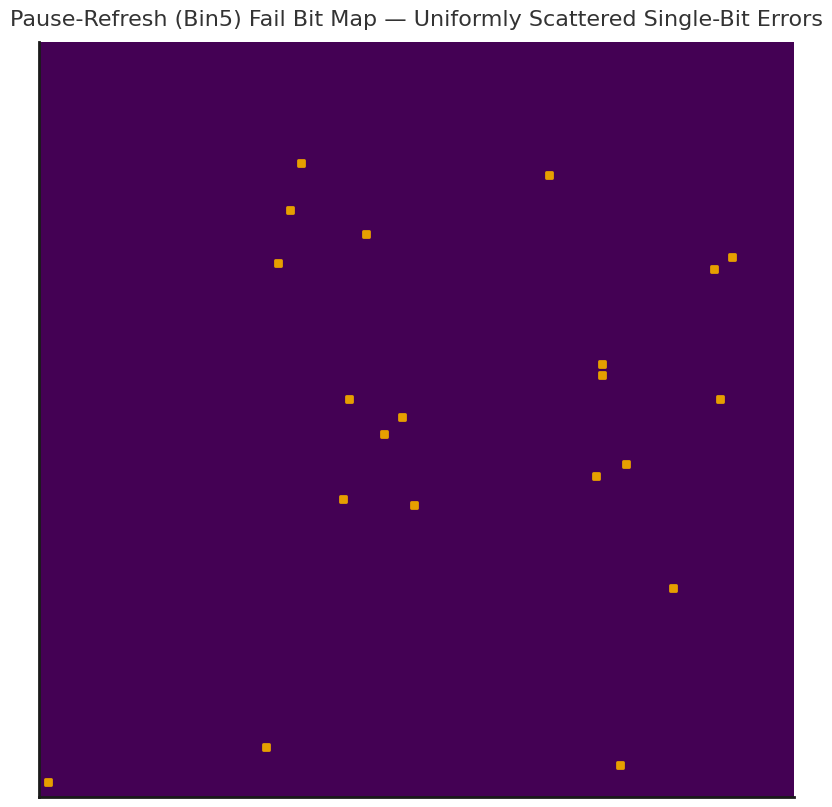
\includegraphics[width=\columnwidth]{fail_bitmap_bin5}
  \caption{Typical fail bit map under pause-refresh test (Bin5).
  Uniformly scattered single-bit errors are observed without edge/line signatures.}
  \label{fig:fail_bitmap}
\end{figure}

\subsection{Hypothesis (Failure Model)}
Directly measurable leakages were normal, suggesting a subtle leakage path. We hypothesized increased leakage at the \textbf{storage-node contact $n^+/p^-$ junction}. After gate etch, a remnant gate oxide on S/D active is repeatedly exposed to resist-stripping \emph{ashing} during multiple LDD steps. Cumulative plasma damage makes the oxide locally porous and can extend damage into the diffusion, creating minute leakage paths. This explains random single-bit distribution without visible structural defects.

% === Storage-node contact n+/p- leakage (TikZ) ===
% === Fig.2 Storage-node contact n+/p- leakage (pure TikZ, minimal IEEE style) ===
\begin{figure}[t]
\centering
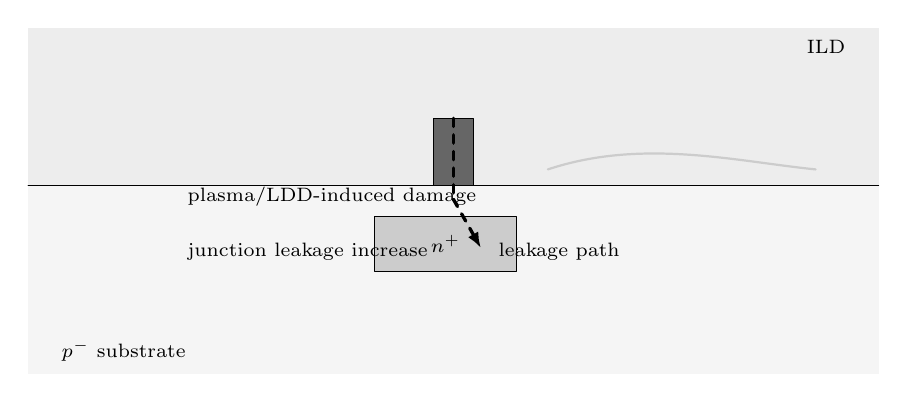
\begin{tikzpicture}[x=1cm,y=1cm,line cap=round,line join=round]
  % 色(グレースケール)
  \def\colILD{black!7}    % ILD淡グレー
  \def\colSub{black!4}    % p-基板の淡グレー
  \def\colDiff{black!20}  % n+拡散
  \def\colLOCOS{black!20} % LOCOS輪郭
  \def\colMetal{black!60} % 金属プラグ

  % キャンバス範囲
  \path (-4.8,-2.4) rectangle (6.0,2.0);

  % ---- ILD(上部帯)----
  \fill[\colILD] (-4.8,0) rectangle (6.0,2.0);
  \node[anchor=east, font=\scriptsize] at (5.7,1.75) {ILD};

  % ---- 基板と表面 ----
  \fill[\colSub] (-4.8,-2.4) rectangle (6.0,0);
  \draw (-4.8,0) -- (6.0,0);
  \node[anchor=west, font=\scriptsize] at (-4.5,-2.1) {$p^{-}$ substrate};

  % ---- LOCOS(右側の鳥のくちばし風プロファイル)----
  \draw[\colLOCOS, line width=0.8pt]
    (1.8,0.20) .. controls (3.0,0.60) and (4.2,0.30) .. (5.2,0.20);

  % ---- n+拡散(ストレージ側)----
  \fill[\colDiff] ( -0.4,-1.1) rectangle (1.4,-0.4);
  \draw ( -0.4,-1.1) rectangle (1.4,-0.4);
  \node[font=\scriptsize] at (0.5,-0.75) {$n^{+}$};

  % ---- ストレージノード・コンタクトプラグ ----
  \fill[\colMetal] (0.35,0.00) rectangle (0.85,0.85);
  \draw (0.35,0.00) rectangle (0.85,0.85);

  % ---- 破線リークパス(コンタクト端→接合)----
  \draw[very thick, dashed] (0.60,0.85) -- (0.60,-0.18);
  \draw[very thick, dashed, -{Latex[length=2mm]}] (0.60,-0.18) -- (0.95,-0.80);
  \node[anchor=west, font=\scriptsize] at (1.05,-0.85) {leakage path};

  % ---- 注記(最小限)----
  \node[anchor=west, font=\scriptsize] at (-2.9,-0.15) {plasma/LDD-induced damage};
  \node[anchor=west, font=\scriptsize] at (-2.9,-0.85) {junction leakage increase};
\end{tikzpicture}
\caption{Schematic of storage-node contact (n$^+$/p$^-$) leakage.
Damage near the contact edge increases junction leakage, degrading retention.}
\label{fig:storage_contact}
\end{figure}

\subsection{Countermeasures}
\begin{itemize}
  \item \textbf{Process}: Replace resist stripping in LDD steps from plasma ashing to \textbf{wet stripping (sulfuric-based)} to eliminate plasma damage. 
  \item \textbf{Integration hygiene}: Confirm downstream photo cleanliness and avoid residue risks with the wet strip.
\end{itemize}

\subsection{Effectiveness}
Yield improved from $\sim$65\% to \textbf{$\sim$80\%}. Uniformly scattered single-bit fails decreased markedly. Burn-in and retention/reliability passed; the final recipe was fixed for volume production.

% === Yield-by-lot (step improvement at countermeasure) ===
\begin{figure}[t]
\centering
\pgfplotstableread[col sep=comma]{data/yield_lot.csv}\yieldtbl
\begin{tikzpicture}
\begin{axis}[
  width=\columnwidth, height=0.58\columnwidth,
  xlabel={Lot ID}, ylabel={Yield [\%]},
  ymin=50, ymax=95,
  xmin=0.5, xmax=12.5,
  grid=both,
  xtick=data,
  xticklabels from table={\yieldtbl}{lot},
  xticklabel style={rotate=45, anchor=east},
]
  % データ描画
  \addplot+[mark=*] table[x expr=\coordindex+1, y=yield]{\yieldtbl};

  % 対策境界: lot04とlot05の間
  \draw[dashed] (axis cs:4.5,50) -- (axis cs:4.5,95);
  \node[anchor=west, font=\footnotesize] at (axis cs:4.55,92)
    {Countermeasure};
\end{axis}
\end{tikzpicture}
\caption{Yield step improvement at the countermeasure boundary
between \texttt{lot04} and \texttt{lot05}. Yield jumps from $\sim$62--63\% 
(lot01--lot04) to $\sim$82--84\% (lot05 onward) after changing 
LDD resist stripping from ashing to wet stripping.}
\label{fig:yield}
\end{figure}

Parallel margin lots efficiently confirmed the process window under mass-line conditions, avoiding delays from strictly serial confirmation. Retention behavior is framed by $\tau = C_{\mathrm{cell}} V_{\mathrm{cell}} / I_{\mathrm{leak}}$, highlighting sensitivity to junction and dielectric leakage. The disturb-refresh behavior connects conceptually to modern row-disturb/row-hammer phenomena. We discuss portability of this ramp-up template to technology transfers beyond DRAM.

% sections/conclusion.tex

DRAM will continue to dominate volatile working memory due to speed, density, and ecosystem maturity. HfO2-based FeRAM/FeFET offers a CMOS-compatible non-volatile complement with fast access, though variability, endurance dispersion, and integration limits remain active topics \cite{noheda2023,martin2020}. Hybrid hierarchies that pair DRAM for hot data with FeRAM for persistence can reduce refresh energy while enabling fast recovery paths.

Looking ahead, co-design across devices, controllers, and operating systems will be central: retention-aware placement, telemetry-driven reliability management, and low-latency persistence paths are promising directions to broaden deployment from embedded and edge to selected data-centric systems.


% ===== Acknowledgment =====
\section*{Acknowledgment}
The author would like to thank the open-source community and educational collaborators
who contributed to the EduController, Edusemi, and AITL projects,
which formed the foundation of this work.

% ===== References =====
\bibliographystyle{IEEEtran}
\nocite{*}  % ★ refs.bib の全エントリを出力(エラー回避)
\bibliography{refs}

% ===== Author Biography =====
\vspace{-0.5\baselineskip}
\begingroup\small
\begin{IEEEbiographynophoto}{Shinichi Samizo}
received the M.S. degree in Electrical and Electronic Engineering from Shinshu University, Japan.
He worked at Seiko Epson Corporation as an engineer in semiconductor memory and mixed-signal device development, and also contributed to inkjet MEMS actuators and PrecisionCore printhead technology.
He is currently an independent semiconductor researcher focusing on process/device education, memory architecture, and AI system integration.

\textbf{Contact:} \href{mailto:shin3t72@gmail.com}{shin3t72@gmail.com},
\href{https://github.com/Samizo-AITL}{Samizo-AITL}
\end{IEEEbiographynophoto}
\endgroup

\end{document}
